\chapter{Sources of Digital Information}
\label{chapter:Sources}

Digital systems use sequences of symbols (e.g., binary systems use 0's and 1's) to represent information.
A \emph{source} of digital information is assumed to produce a succession of symbols, each drawn from a \emph{discrete alphabet}.
The three goals of this chapter are to understand the nature of digital information, find an adequate measure of information for digital systems and to describe compression algorithms that can be employed to represent the said information in a succinct manner.
\emph{Data compression}, also known as \textbf{source coding}, is important because it reduces the consumption of expensive resources such as hard disk space or transmission bandwidth.
Alternatively, it can be applied to lower the cost of communication, reduce latency or improve the quality of the received messages.

This document offers an introductory treatment of \emph{lossless compression} algorithms, whereby the original message can be recovered perfectly from the compressed data.
This is in contrast to \emph{lossy data compression}, which can achieve better compression ratio at the expense of introducing some distortion in the message.
In the latter case, part of the information may be lost and the original data need not be perfectly recoverable, although the reconstructed message may be quite close to the original one.
For instance, the JPEG algorithm can be employed as a lossy compression scheme to reduce the size of a digital photograph.
In lossless data compression, two strategies are employed to reduce the expected length of a message.
Highly probable symbols are assigned short descriptions, and less likely symbols are encoded using longer binary representations.
Second, the statistical redundancy contained in the input signal over time is removed, leading to a more concise description of the digital data.
Data compression algorithms are explained more thoroughly below.

As we will see, finding a pertinent measure of information is key in assessing the performance and limitations of compression algorithms.
While the general notion of information may be quite broad, it has a precise definition in the context of digital communication systems.
To describe this specific meaning, we first need to develop a rigorous mathematical model for digital information sources.


\section{Discrete Memoryless Sources}

As mentioned above, a digital source produces a sequence of symbols drawn from a countable alphabet.
It can accordingly be modeled as a discrete-time random process.
Because of their indeterminate nature, random signals and stochastic processes can be quite hard to characterize.
In early sections of this document, we discussed two desirable attributes of random signals, namely stationary and ergodicity.
Yet, we purposely avoided giving an explicit definition for a random process.
A detailed discussion of the subject requires advanced concepts from probability theory, a topic that interested readers may wish to pursue on their own.
For the sake of simplicity, we focus on a class of elementary information sources that are collectively known as discrete memoryless sources.
These sources are easy to analyze and can be described unambiguously in a straightforward manner.
Furthermore, discrete memoryless sources provide valuable insights into the design of efficient compression algorithms for more general settings.

\begin{definition}
A \defn{source coding}{discrete memoryless source} is a digital information source that produces a sequence of independent and identically distributed symbols over time.
Mathematically, it consists of an alphabet $\mathcal{X}$ and a probability mass function $p_X(\cdot)$ such that, at any time~$t$, the probability that the source outputs symbol $x \in \mathcal{X}$ is equal to $p_X(x)$, irrespective of the past and future.
\end{definition}

For discrete memoryless sources, it suffices to define the probability mass function of individual symbols to completely characterize the statistical properties of the corresponding random signal.
The higher-order statistics need not be specified explicitly, as they can be obtained from
\begin{equation} \label{equation:JointDistributionMemorylessSource}
\Pr (X_{t_1} = x_{t_1}, \ldots, X_{t_n} = x_{t_n})
= \prod_{k = 1}^n p_X(x_{t_k})
\end{equation}
where $x_{t_1}, \ldots, x_{t_n} \in \mathcal{X}$.
In \eqref{equation:JointDistributionMemorylessSource}, the random variable $X_{t_i}$ denotes the output of the source at time~$t_i$.
We provide two examples of memoryless sources below to further illustrate their form.

\begin{example}[Binary Source] \label{example:BinarySource}
The simplest possible information source is a discrete memoryless source where $p_X(\cdot)$ is the probability mass function of a Bernoulli random variable,
\begin{equation*}
p_X(x) = \begin{cases} (1 - p), & x = 0 \\
p, & x = 1 \end{cases}
\end{equation*}
with $p \in [0,1]$.
This source can be employed, for instance, to model the successive flipping of a biased coin, where heads is obtained with probability $p$ and tails is obtained with probability $1 - p$.
\end{example}

\begin{example}
To construct a slightly more elaborate example, consider a collection of experiments where a fair coin is flipped repetitively until heads is observed.
The outcome of each experiment is reported as a source output.
The source alphabet in this case is $\mathcal{X} = \{1, 2, \ldots \}$, the positive integers, and the marginal probability mass function associated with individual outcomes becomes
\begin{equation*}
p_X (x) = \frac{1}{2^x}, \quad x = 1, 2, \ldots
\end{equation*}
Thus, the distribution of the source output at time~$t$ is a geometric random variable with parameter~$\frac{1}{2}$.
\end{example}

It is straightforward to show that all discrete memoryless sources are both stationary and ergodic.
The fact that their outcomes are independent over time makes them convenient for analysis, leading to simple interpretations.
However, it should also be pointed out that many realistic sources are more complicated than memoryless sources.
In particular, their outputs may be correlated over time, which can have a major impact on information rates.
Handling intricate sources requires heavy mathematical machinery, and is beyond the scope of this document.
The results derived using more involved sources are, nevertheless, similar in nature to the ones presented below.
This partially explains why we choose not to study more difficult information sources in this document.

Having constructed a suitable abstraction for digital sources, we turn to the subject of digital information.
From an intuitive point of view, the data rate of a discrete memoryless source should be equal to the amount of information it produces at every time instant.
In other words, the amount of information created by a discrete memoryless source at time~$t$ should be computable based on $\mathcal{X}$ and $p_X(\cdot)$ exclusively.
This is indeed the case.
Before we can make this statement precise, we need a rigorous mathematical characterization of information.
We address this issue by introducing entropy, a concept closely related to the notion of information.


\section{Entropy}

The \defn{information theory}{entropy} can be viewed as a measure of uncertainty in a random variable.
In the context of digital communications, it serves as a measure of information in that it provides a lower bound on the expected number of bits required to describe the output of a discrete memoryless source.
This lower bound is tight and can be approached using various schemes, as we will see shortly.

\begin{definition}[Entropy]
Let $X$ be a discrete random variable drawn from alphabet $\mathcal{X}$ according to probability mass function $p_X(\cdot)$.
The entropy of $X$, denoted $\mathrm{H}[X]$, is given by
\begin{equation} \label{equation:Entropy}
\mathrm{H}[X] = - \sum_{x \in \mathcal{X}} p_X (x) \log_2 ( p_X(x) ) .
\end{equation}
Under this definition, entropy is described in bits.
When writing $\mathrm{H}[X]$, we use the convention
\begin{equation*}
0 \cdot \log_2 \left( \frac{1}{0} \right)
= \lim_{\epsilon \rightarrow 0} \epsilon \log_2 \left( \frac{1}{\epsilon} \right)
= 0 .
\end{equation*}
Alternatively, the entropy of $X$ can be interpreted as the expectation of a logarithmic function,
\begin{equation*}
\mathrm{H}[X] = \mathrm{E} \left[ \log_2 \left( \frac{1}{p_X(X)} \right) \right] .
\end{equation*}
\end{definition}

The entropy as described in \eqref{equation:Entropy} has interesting properties.
The value $\mathrm{H}[X]$ does not depend on the actual symbols themselves, it only depends on the probability mass function of the possible outcomes.
For instance, in Example~\ref{example:EntropyFairCoin}, the entropy of $X$ remains the same whether we represent the flipping of a coin by a single bit or through a string of letters, heads or tails.
More generally, the way we choose to designate the possible outcomes of a random experiment has no bearing over the entropy of the corresponding source, only the respective probabilities of the possible symbols matter.

\begin{example} \label{example:EntropyFairCoin}
Let $X$ be an abstract representation of the flipping of a (possibly biased) coin.
The probability mass function of $X$ is then equal to
\begin{equation*}
p_X(x) = \begin{cases} (1-p), & x = 0 \\
p, & x = 1 \end{cases}
\end{equation*}
with zero denoting tails and one for heads.
We can compute the entropy of $X$ as follows,
\begin{equation*}
\mathrm{H}[X] = - (1-p) \log_2 (1-p)
- p \log_2 (p) .
\end{equation*}
If the coin is fair, $p = \frac{1}{2}$, then the entropy of $X$ becomes one  bit.
Hence, the minimum expected number of bits needed to describe the outcome of a fair coin toss is one.
This seems quite reasonable.
\end{example}

%
% plot of binary entorpy needed.
%

The entropy of pair of two independent random variables is the sum of the individual entropies.
Suppose that $X$ is a vector random variable given by $X = (U, V)$, where $U$ and $V$ are independent.
Then, we can write
\begin{equation*}
p_X(x) = p_X((u, v)) = p_{U} (u) p_{V} (v)
\end{equation*}
and the entropy of $X$ can be computed as
\begin{equation*}
\begin{split}
\mathrm{H}[X] &= - \sum_{ x \in \mathcal{X} } p_X(x) \log_2 ( p_X(x) ) \\
&= - \sum_{(u, v) \in \mathcal{U} \times \mathcal{V}}
p_X((u, v)) \log_2 ( p_X((u, v)) ) \\
&= - \sum_{u \in \mathcal{U}} \sum_{v \in \mathcal{V}}
p_{U} (u) p_{V} (v) \log_2 ( p_{U} (u) p_{V} (v) ) \\
&= - \sum_{u \in \mathcal{U}}
p_{U} (u) \log_2 ( p_{U} (u) )
- \sum_{v \in \mathcal{V}}
p_{V} (v) \log_2 ( p_{V} (v) ) \\
&= \mathrm{H}[U] + \mathrm{H}[V] .
\end{split}
\end{equation*}
This corresponds to our intuitive understanding; the amount of information contained in two unrelated events should be the sum of the information pertaining to each individual event.

It is important to recognize that $\mathrm{H}[X]$ is computed based on the probability mass function $p_X(\cdot)$, it is not a function of the random variable $X$ itself.
As such, $\mathrm{H}[X]$ is a deterministic quantity and does not depend on the actual realization of $X$.
Furthermore, we note that $\mathrm{H}[X]$ is continuous in the weights of the distribution $p_X(\cdot)$.
A small change in the distribution of $X$ only results in a small variation in its entropy.
It is therefore possible to construct accurate entropy estimates based on empirical measurements of the source outputs.


\section{Variable-Length Compression Codes}

A \defn{source coding}{code} is a rule for converting a symbol (or a group of symbols) into a string of bits called a \defn{source coding}{codeword}.
Mathematically, an encoder is a mapping $c : \mathcal{X} \mapsto \mathcal{C}$ from the input alphabet $\mathcal{X}$ to the collection of possible codewords $\mathcal{C}$.
The goal of a \defn{source coding}{compression code} is, of course, to provide a more concise representation of the information signal.
In lossless compression, the function $c$ must be injective over the support of $X$.
Without this one-to-one relationship, decoding errors are bound to happen.
Encoding schemes can be partitioned into two categories based on the structure of their codebooks.
If the codewords all share the same bit-length, then the corresponding code is called a \defn{source coding}{fixed-length code}.
This section focuses on codes in the second category, variable-length codes, which are often used in lossless data compression.

As the name suggests, a \defn{source coding}{variable-length code} is an encoding function that maps source symbols to a variable number of bits.
This is a beneficial feature for many compression schemes, as the greater flexibility sometimes leads to better compression ratio.
The motivation behind variable-length encoding is the intuition that data compression can be achieved by assigning short bit strings to likely symbols, and necessarily longer bit strings to less probable ones.
In dealing with variable-length codes, it is essential to recognize that they are inherently more tricky than fixed-length ones.
With variable-length coding, it may be impossible to know where codewords begin in a compressed binary file without knowing the content of the file.
This is in stark contrast with fixed-length codes where codewords are positioned at regular intervals and, therefore, easy to distinguish.
To ensure that the binary output of a variable-length encoder can be recovered unambiguously, the code needs specific properties.

Variable-length codes can be nested in order of decreasing generality as non-singular, uniquely decodable and instantaneous.
A code is \defn{source coding}{non-singular} if each source symbol is mapped to a different bit string.
That is, the mapping $c$ from $\mathcal{X}$ to $\mathcal{C}$ is one-to-one.
Rather, if two symbols map to the same codeword, then it is intuitively clear that the original message cannot be recovered with certainty.
A code is said to be \defn{source coding}{uniquely decodable} if its extensions are non-singular.
The extension of a code $c$ is obtained by concatenating its codewords when $c$ is applied to a multitude of source symbols.
Given the string of symbols $x_1, x_2, \ldots, x_n$, the extension of $c$ produces the output bit string
\begin{equation*}
c(x_1) c(x_2) \cdots c(x_n) .
\end{equation*}
An extension of $c$ is a proper encoding schemes because it takes a group of symbols as its argument and produces a string of bits as its output.

It is important to recognize that successive codewords in a message are communicated as an undifferentiated sequence of bits.
There is no separation marker or frame between adjacent codewords, no commas or spaces.
The decoder, given a starting point, must infer the boundaries of every codeword from the data.
This process is called \emph{parsing}.
The third and final property of variable-length encoding is related to parsing.
A code is \emph{instantaneous}, or \defn{source coding}{prefix-free}, if no codeword in $\mathcal{C}$ is a prefix of a any other encoded symbol in $\mathcal{C}$.
This property guarantees that each encoded symbol can be identified with no further delay once the corresponding string of bits is received or read.

\begin{example}
Suppose that a source produces three possible symbols, $\mathcal{X} = \{ x_1, x_2, x_3 \}$.
We consider four encoding functions ($c_1, c_2, c_3, c_4$), each with different properties.
The encoding schemes are defined as follows.

\begin{center}
\begin{tabular}{|c|c|c|c|c|}
\hline
Symbol & \multicolumn{4}{c|}{Codeword} \\
\hline
$x$ & $c_1(x)$ & $c_2(x)$ & $c_3(x)$ & $c_4(x)$ \\
\hline
$x_1$ & 0 & 0 & 0 & 0 \\
$x_2$ & 1 & 1 & 01 & 10 \\
$x_3$ & 0 & 01 & 11 & 11 \\
\hline
\end{tabular}
\end{center}

The first scheme is not injective because it maps two different source symbols to the same codeword, $c_1(x_1) = c_1(x_3)$.
Thus, individual codewords cannot be decoded unambiguously.
The second code is one-to-one; however, it is not uniquely decodable.
The encoded message 01 can be generated by either input string $x_1 x_2$ or input symbol $x_3$.
Clearly, the compressed message is not uniquely decodable.
The third code, $c_3(\cdot)$ is uniquely decodable, but not instantaneous.
After receiving a zero, it not immediately clear whether $x_1$ produced this output or if this zero consists of the first half of codeword $c(x_2)$.
While $c_4(\cdot)$ is a prefix code where every symbol can be decoded immediately after reading the corresponding bits.
\end{example}

The measure of a good prefix code is the expected length of its encoded symbols.
Suppose that a discrete memoryless source $(\mathcal{X}, p_X)$ is given along with a code $c$.
We denote the length in bits of codeword $c(x)$ by $\ell_c(x)$.
The expected number of bits produced by the source at each time instant is given by
\begin{equation} \label{equation:CodeRateCompression}
\mathrm{E} [ \ell_c (X) ] = \sum_{x \in \mathcal{X}} p_X(x) \ell_c(x) .
\end{equation}
We emphasize that the expected length is a function of both the statistics of the source and the structure of compression code employed.
Under the assumption that the source outcomes are independent and identically distributed over time, $\mathrm{E} [ \ell_c (X)]$ also represents the average data rate produced by the source, in bits per source symbol.


\subsection{Kraft Inequality}

When building a compression code, it is obvious from \eqref{equation:CodeRateCompression} that assigning short codewords is better than long codewords.
Yet, it is clear that we cannot describe every symbol using a very small number of bits, for otherwise the prefix condition will be violated.
The collection of possible length assignments for a prefix-free code is characterized by the following inequality.

\begin{theorem}[Kraft Inequality]
Let $\mathcal{X}$ be a finite alphabet.
Any binary prefix-free code $c : \mathcal{X} \mapsto \mathcal{C}$ satisfies the inequality
\begin{equation} \label{equation:KraftInequality}
\sum_{x \in \mathcal{X}} 2^{-\ell_c(x)} \leq 1.
\end{equation}
where $\ell_c(x)$ is the bit length of codeword $c(x)$.
Conversely, if we first assign the codeword lengths such that \eqref{equation:KraftInequality} is satisfied, then there exists an instantaneous code with these codeword lengths.
\end{theorem}
\begin{proof}
We wish to give necessary and sufficient conditions about the existence of a prefix-free code with a specific length assignment.
We employ simple combinatorial arguments to a binary tree structure to establish this result.
\begin{figure}[htbp]
\begin{center}
\begin{psfrags}
\psfrag{0}[c]{$0$}
\psfrag{1}[c]{$1$}
\psfrag{C0}[l]{$000$}
\psfrag{C1}[l]{$001$}
\psfrag{C2}[l]{$010$}
\psfrag{C3}[l]{$011$}
\psfrag{C4}[l]{$100$}
\psfrag{C5}[l]{$101$}
\psfrag{C6}[l]{$110$}
\psfrag{C7}[l]{$111$}
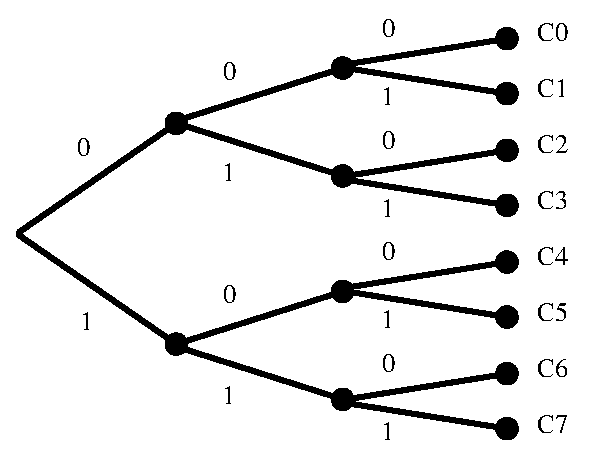
\epsfig{file=Figures/binarytree,width=7cm}
\end{psfrags}
\caption{This figure shows a binary tree with depth $L_c = 3$ and eight leaves.  The branches from every node correspond to zero or one.}
\label{figure:BinaryTree}
\end{center}
\end{figure}
Let $L_c = \max_{x \in \mathcal{X}} \ell_c (x)$ be the length of the longest codeword.
Code $c: \mathcal{X} \mapsto \mathcal{C}$ can be defined using a binary tree of depth $L_c$, where branches from every node correspond either to zero or one.
Each codeword consists of a unique path from the root to a leaf at depth $\ell_c(x)$, following its binary string expansion.
The prefix condition ensures that no codeword is a descendant of any other codeword in the binary tree.
For the codewords in the tree, let $S_x$ be the set of descendants that $c(x)$ would have in a full binary tree of depth $L_c$.
The sets $S_x$ are disjoint because of the prefix-free nature of the code, and $|S_x| = 2^{L_c - \ell_c(x)}$.
Since the total number of nodes at depth $L_c$ is $2^{L_c}$, we have
\begin{equation*}
\left| \bigcup_{x \in \mathcal{X}} S_x \right|
= \sum_{x \in \mathcal{X}} |S_x|
= \sum_{x \in \mathcal{X}} 2^{L_c - \ell_c(x)}
\leq 2^{L_c} .
\end{equation*}
By dividing both sides by $2^{L_c}$, we conclude that \eqref{equation:KraftInequality} holds.
That is, a binary prefix-free code $c$ over finite alphabet $\mathcal{X}$ satisfies the Kraft inequality.

Conversely, suppose that we have a code assignment such that \eqref{equation:KraftInequality} is satisfied.
Without loss of generality, we assume that the codeword lengths $\ell_c(x_i)$ are increasing in~$i$,
\begin{equation*}
\ell_c(x_1) \leq \ell_c(x_2) \leq \ell_c(x_3) \leq \cdots
\end{equation*}
We can construct a prefix code with matching codeword lengths by pruning subtrees from a  full binary tree of depth $L_c$.
First, choose any node from the full tree at depth $\ell_1$ and remove all of its descendants.
This removes $2^{L_c -\ell_1}$ leafs from the original binary tree.
Next, select any available node from the resulting tree at depth $\ell_2$, and remove all of its descendants.
This time, an additional $2^{L_c - \ell_2}$ leafs are taken away from the original binary tree.
Continue this procedure with the other codeword lengths.
After $m$ iterations, the total number of leafs removed from the original binary tree is equal to
\begin{equation*}
\sum_{i=1}^m 2^{L_c - \ell_i} = 2^{L_c} \sum_{i=1}^m 2^{-\ell_i} .
\end{equation*}
Since the Kraft inequality holds for the codeword length assignment, this implies that all the codewords can be placed at different positions on the binary graph.
Then, following the binary structure of the graph, the binary string of the codes can be inferred from the graph.
\end{proof}

\begin{example}[Code on a Tree]
Suppose that we intend to construct a prefix code for $\mathcal{X} = \{ x_1, \ldots, x_5 \}$, with code lengths
\begin{xalignat*}{3}
\ell_c(x_1) &= \ell_c(x_2) = 2 & \ell_c(x_3) &= \ell_c(x_4) = 3 & \ell_c(x_5) &= 2.
\end{xalignat*}
First, we check the Kraft inequality to make sure that such an assignment is feasible,
\begin{equation*}
\sum_{i = 1}^5 2^{-\ell_c(x_1)}
= \frac{1}{4} + \frac{1}{4} + \frac{1}{8} + \frac{1}{8} + \frac{1}{4} = 1 .
\end{equation*}
The inequality is fulfilled, we can therefore use a binary tree construction to design the desired instantaneous code.
The process is illustrated in Figure~\ref{figure:BinaryTreeCode}, and the resulting code is shown below.

\begin{center}
\begin{tabular}{|c|c|c|c|}
\hline
Source Symbol & Codeword & Source Symbol & Codeword \\
\hline
$x_1$ & 00 & $x_4$ & 101 \\
$x_2$ & 01 & $x_5$ & 11 \\
$x_3$ & 100 & & \\
\hline
\end{tabular}
\end{center}

Since the Kraft inequality is met with equality, we know that it is impossible to get a better code by shortening one of the codewords.
\begin{figure}[htbp]
\begin{center}
\begin{psfrags}
\psfrag{0}[c]{$0$}
\psfrag{1}[c]{$1$}
\psfrag{00}[l]{$00$}
\psfrag{01}[l]{$01$}
\psfrag{100}[l]{$100$}
\psfrag{101}[l]{$101$}
\psfrag{11}[l]{$11$}
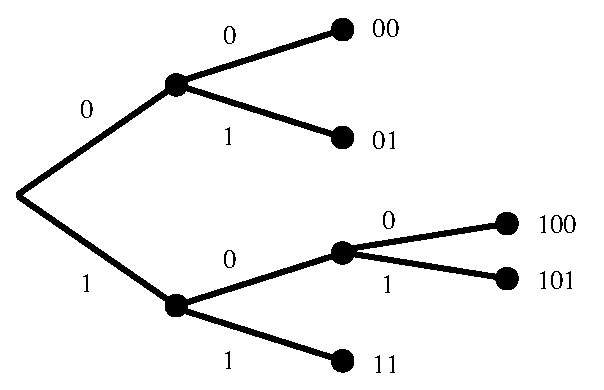
\epsfig{file=Figures/binarytreecode,width=7cm}
\end{psfrags}
\caption{Construction of a prefix code with a binary tree.}
\label{figure:BinaryTreeCode}
\end{center}
\end{figure}
\end{example}


\subsection{Entropy Bounds on Prefix-Free Codes}

Now that we know how to build instantaneous, we consider the problem of finding good prefix-free codes.
Recall from \eqref{equation:CodeRateCompression} that our objective is to find a prefix-free code with the smallest possible expected length.
As seen earlier, this codeword length assignment is subject to the Kraft inequality.
Putting these two requirements together, we can formulate the optimization problem as follows,
\begin{equation*}
\min_{\ell(x)} \sum_{x \in \mathcal{X}} p_X(x) \ell(x)
\quad \text{subject to} \quad
\sum_{x \in \mathcal{X}} 2^{- \ell(x)} \leq 1 .
\end{equation*}
We note that, for a code to exist, the function $\ell(x)$ must take values in the positive integers.
It turns out that this problem is difficult to solve.

To gain insight into the problem, we relax the integer constrain on $\ell(x)$.
This added flexibility will provide a lower bound on $\mathrm{E} [\ell(X)]$; having more choices can only lead to better results.
We use the method of Lagrange multipliers to solve the latter version of the problem.
The objective function, with Lagrange multiplier $\lambda$, becomes
\begin{equation*}
\sum_{x \in \mathcal{X}} p_X(x) \ell(x)
+ \lambda \left( \sum_{x \in \mathcal{X}} 2^{- \ell(x)} - 1 \right) .
\end{equation*}
Note that this function is twice differentiable in $\ell(x)$.
Taking a partial derivative with respect to $\ell(x)$ and setting it to zero, we get
\begin{equation*}
p_X(x) - \lambda \ln(2) 2^{- \ell(x)}  = 0 .
\end{equation*}
The optimal value for $\ell(x)$, which we denote by $\ell^{\star}(x)$, must therefore satisfy $2^{- \ell^{\star}(x)} = p_X(x) / (\lambda \ln (2))$.
Computing the derivative with respect to $\lambda$ yields
\begin{equation*}
\sum_{x \in \mathcal{X}} 2^{- \ell^{\star}(x)} = 1 ,
\end{equation*}
which in turn implies $\lambda = 1 / \ln (2)$.
Putting these results together, we gather that the optimal values for $\{ \ell(x) : x \in \mathcal{X} \}$ are given by
\begin{equation*}
\ell^{\star}(x) = - \log_2 (p_X(x))
\end{equation*}
for $x \in \mathcal{X}$.
Thus, by construction, we obtain
\begin{equation*}
\mathrm{E} [\ell_c(X)] \geq - \sum_{x \in \mathcal{X}} p_X(x) \log_2 (p_X(x))
= \mathrm{H}[X]
\end{equation*}
for any prefix-code~$c$.
In other words, the entropy is a lower bound on the expected length of any prefix-free code.

It is equally easy to obtain an upper bound on the expected length of an optimal prefix-free code.
Observe that $\lceil - \log_2 (p_X(x)) \rceil$ is an integer, with
\begin{equation*}
- \log_2 (p_X(x))
\leq \lceil - \log_2 (p_X(x)) \rceil
\leq - \log_2 (p_X(x)) + 1 .
\end{equation*}
The Kraft inequality asserts that we can build a code $c : \mathcal{X} \mapsto \mathcal{C}$ such that $\ell_c(x) = \lceil - \log_2 (p_X(x)) \rceil$, as
\begin{equation*}
\sum_{x \in \mathcal{X}} 2^{- \ell_c(x)}
\leq \sum_{x \in \mathcal{X}} 2^{- \ell^{\star}(x)} = 1 .
\end{equation*}
As such, there exists a code~$c$ such that
\begin{equation*}
\mathrm{E} [\ell_c(X)] \leq \mathrm{H}[X] + 1 .
\end{equation*}
We collect and formalize these important results in the form of a theorem.

\begin{theorem} \label{theorem:EntropyBoundsPrefixCodes}
Consider a discrete memoryless source $(\mathcal{X}, p_X(\cdot))$ over a finite alphabet.
If symbols are encoded individually using an optimal prefix-free code $c : \mathcal{X} \mapsto \mathcal{C}$, then the expected length of the codewords satisfies
\begin{equation*}
\mathrm{H}[X] \leq \mathrm{E} [\ell_c(X)] \leq \mathrm{H}[X] + 1 .
\end{equation*}
\end{theorem}


\subsection{Huffman Codes}

Theorem~\ref{theorem:EntropyBoundsPrefixCodes} identifies properties of an optimal prefix-code.
However, it does not provide an algorithmic methodology to design such a code.
This is addressed by the \defn{source coding}{Huffman code}, which provides an efficient variable-length code for lossless data compression.
Not too surprisingly, the underlying strategy in this scheme is to assign short strings of bits to likely symbols, and necessarily longer ones to less probable source outputs.
The encoding is specifically crafted so that the code table forms a prefix-free code.
Huffman codes are the most efficient compression mapping for individual source symbols.
The expected length of the compressed data achieved with this technique will be no greater than the expected message length of any other prefix-free code that operates on individual source symbols.

The insight behind Huffman coding is based on three properties of optimal prefix-codes.
Suppose that we wish to encode outputs from discrete memoryless source $(\mathcal{X}, p_X)$, and let $c^{\star} : \mathcal{X} \mapsto \mathcal{C}$ be an optimal prefix-code for this source.
If $p_X(x_1) > p_X(x_2)$, then $\ell_{c^{\star}}(x_1) \leq \ell_{c^{\star}}(x_2)$.
For any of the longest codewords, its sibling (the bit string that differs only in the last digit) must also be codeword; otherwise, the original codeword can be shortened by removing the last bit.
Finally, the code tree associated with an optimal code must be full.
A binary tree is \emph{full} if every node has either zero or two children.
Again, if this condition fails, then some codewords in the codebook can be shortened.

The Huffman algorithm creates a code by building a binary tree.
The algorithm proceeds as follows.
First, every source symbol $x$ is assigned to an individual node.
Then, the simple recursion outlined below is applied.
\begin{enumerate}
\item Sort the nodes in decreasing order of probabilities.
\item Merge the two least probable nodes into a single one, whose probability equals the sum of its constituents.
\item Arbitrarily assign zero or one to the branches emerging from this new node.
\item Repeat the previous three steps with the new collection of nodes and their corresponding probabilities until only one node remains.
\end{enumerate}
The Huffman encoding algorithm is best grasped through simple examples.

\begin{example}
Suppose that a discrete memoryless source $(\mathcal{X}, p_X)$ with alphabet $\mathcal{X} = \{ x_1, x_2, x_3 \}$ has probability mass function
\begin{equation*}
p_X(x) = \begin{cases} \frac{2}{3}, & x = x_1 \\
\frac{1}{6}, & x \in \{ x_2, x_3 \} . \end{cases}
\end{equation*}
We wish to obtain an optimal prefix-code for this source, and thus we apply the Huffman algorithm.
For the given source, code design proceeds as follows.

\begin{center}
\begin{tabular}{|c|c|c|c|c|}
\hline
Stage 3 & Stage 2 & Stage 1 & Symbol & Codeword \\
\hline
$\Pr \{ x_1, x_2, x_3 \} = 1$ & $\Pr \{ x_1 \} = \frac{2}{3}$
& $p_X (x_1) = \frac{2}{3}$ & $x_1$ & 0 \\
& $\Pr \{ x_2, x_3 \} = \frac{1}{3}$ & $p_X (x_2) = \frac{1}{6}$ & $x_2$ & 10 \\
& & $p_X (x_3) = \frac{1}{6}$ & $x_3$ & 11 \\
\hline
\end{tabular}
\end{center}

From this successive re-ordering of probabilities, we use a binary tree to build the actual code.
This is illustrated in Figure~\ref{figure:Huffman1}.
\begin{figure}[htbp]
\begin{center}
\begin{psfrags}
\psfrag{C1}[l]{$0$}
\psfrag{C2}[l]{$10$}
\psfrag{C3}[l]{$11$}
\psfrag{x1}[c]{$x_1$}
\psfrag{x2}[c]{$x_2$}
\psfrag{x3}[c]{$x_3$}
\psfrag{x23}[c]{$\{ x_2, x_3 \}$}
\psfrag{x123}[c]{$\{ x_1, x_2, x_3 \}$}
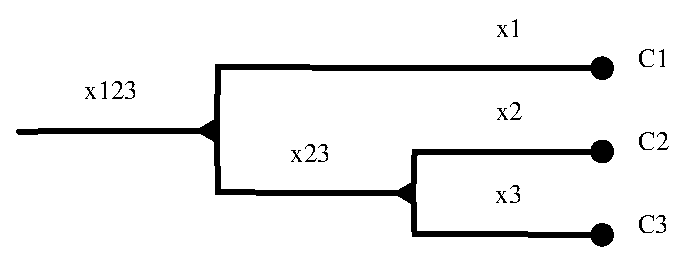
\epsfig{file=Figures/huffman1,width=68.718mm}
\end{psfrags}
\caption{A graphical representation for the construction of a simple Huffman code. The source alphabet in this case is $\mathcal{X} = \{x_1, x_2, x_3 \}$ and the probabilities of individual symbols are $\{ 2/3, 1/6, 1/6 \}$, respectively.}
\label{figure:Huffman1}
\end{center}
\end{figure}
\end{example}

\begin{example}
A source $(\mathcal{Y}, p_Y)$ generates four different symbols $\{ y_1, y_2, y_3, y_4 \}$ with probabilities $\{ 0.35, 0.25, 0.2, 0.2 \}$.
A binary tree is generated from right to left, by merging the two less probable symbols at every step.
Once this is complete, the code can then be form by assigning different bits to every pair of branches emerging from a node.
The table below shows the different stages of the iterative procedure where probabilities are first sorted in decreasing order, then the two least probable nodes are merged into a single one.

\begin{center}
\begin{tabular}{|c|c|c|c|}
\hline
Stage 4 & Stage 3 & Stage 2 & Stage 1 \\
\hline
$0.6 + 0.4 = 1$ & $0.35 + 0.25 = 0.6$ & $0.2 + 0.2 = 0.4$ & $p_X (x_1) = 0.35$ \\
& $0.4$ & $0.35$ & $p_X (x_2) = 0.25$ \\
& & $0.25$ & $p_X (x_3) = 0.2$ \\
& & & $p_X (x_4) = 0.2$ \\
\hline
\end{tabular}
\end{center}

The ensuing Huffman code is obtained by moving from left to right in the corresponding binary tree.
The binary tree and the resulting Huffman code are shown in Figure~\ref{figure:Huffman2}.

\begin{figure}[htbp]
\begin{center}
\begin{psfrags}
\psfrag{C1}[l]{$00$}
\psfrag{C2}[l]{$01$}
\psfrag{C3}[l]{$10$}
\psfrag{C4}[l]{$11$}
\psfrag{x1}[c]{$x_1$}
\psfrag{x2}[c]{$x_2$}
\psfrag{x3}[c]{$x_3$}
\psfrag{x4}[c]{$x_4$}
\epsfig{file=Figures/huffman2,width=87.791mm}
\end{psfrags}
\caption{This figure depicts a Huffman code construction for an alphabet of size four.}
\label{figure:Huffman2}
\end{center}
\end{figure}

\end{example}

Although Huffman coding is optimal for a symbol-by-symbol encoding with a known input probability mass function, it can be outperformed when these two conditions are not known.
For instance, if the input distribution $p_X(\cdot)$ is not known, then it must be inferred from the available data prior to applying Huffman coding.
Small errors in the estimated probability mass function can then lead to inefficiency, which in turn renders Huffman coding suboptimal.
We will soon see an encoding algorithm that does not require the input distribution $p_X(\cdot)$.
However, before we can present this algorithm, we need to consider the join encoding of source symbols.


\section{Joint Encoding of Source Symbols}

Under special circumstances, namely when the probability of every source symbol is an exponent base two, the expected length of a Huffman code is equal to the entropy of the source.
However, in many situations, this is not the case, and there exists a gap between the expected codeword length and the entropy of a source output.
An efficient way to encode data, where the expected number of coded bits per source symbol approaches the entropy, is to consider blocks of source symbols and to encode them jointly.
Although more complicated, this process leads to better performance and typically leads to expected message lengths that are shorter  than that of a symbol-by-symbol Huffman code.

Consider a sequence $X_1, X_2, \ldots$ of symbols at the output of a discrete memoryless source.
Instead of using a code that operates on individual symbols, we can design a more elaborate code that takes as input a group of $n$ symbols, $c: \mathcal{X}^n \mapsto \mathcal{C}$.
Since the outputs of a discrete memoryless source are independent and identically distributed random variables, we know from the additive property of the entropy that
\begin{equation*}
\mathrm{H}[X_1, \ldots, X_n ] = n \mathrm{H} [X] .
\end{equation*}
Then, by applying Theorem~\ref{theorem:EntropyBoundsPrefixCodes}, we get that an optimal prefix code, which operates on $\mathcal{X}^n$, yields
\begin{equation*}
n \mathrm{H}[X] \leq \mathrm{E} [ \ell_c (X_1, \ldots, X_n) ] \leq n \mathrm{H}[X] + 1.
\end{equation*}
Then, the expected message length per source output becomes
\begin{equation*}
\mathrm{H}[X] \leq \frac{ \mathrm{E} [ \ell_c (X_1, \ldots, X_n) ] }{n} \leq \mathrm{H}[X] + \frac{1}{n} .
\end{equation*}
Thus, the expected number of bits per symbol produced by a source can be made arbitrarily close to $\mathrm{H}[X]$ by jointly encoding strings of symbols.

\begin{example} \label{example:JointSourceCoding}
Let $(\mathcal{X}, p_X)$ be a binary discrete memoryless source, as described in Example~\ref{example:BinarySource}.
Furthermore, assume that Bernoulli parameter $p$ is equal to $\frac{1}{4}$.
Then, the entropy of the source can be calculated as
\begin{equation*}
\mathrm{H}[X] = - \frac{3}{4} \log_2 \left( \frac{3}{4} \right)
- \frac{1}{4} \log_2 \left( \frac{1}{4} \right)
\approx 0.811 .
\end{equation*}
Since there are only two source symbols, a code generated by the Huffman algorithm is the identity code, where a source output is represented by its binary value.
In this case, the expected codeword length is equal to one.

Suppose instead that two symbols are encoded at a time.
In this case, the possible inputs to the encoder are $\{ 00, 01, 10, 11 \}$, with respective probabilities $\left\{ \frac{9}{16}, \frac{3}{16}, \frac{3}{16}, \frac{1}{16} \right\}$.
The Huffman code specified by
\begin{center}
\begin{tabular}{|c|c|c|c|c|}
\hline
Symbol & Codeword \\
\hline
$00$ & 0 \\
$01$ & 10 \\
$10$ & 110 \\
$11$ & 111 \\
\hline
\end{tabular}
\end{center}
has an expected length of
\begin{equation*}
\mathrm{E} [\ell_c (X_1, X_2)] = 1 \cdot \frac{9}{16} + 2 \cdot \frac{3}{16}
+ 3 \cdot \frac{3}{16} + 3 \cdot \frac{1}{16}
= \frac{27}{16} . 
\end{equation*}
The expected message length per source output becomes
\begin{equation*}
\frac{\mathrm{E} [\ell_c (X_1, X_2)]}{2} = \frac{27}{32} \approx 0.844 ,
\end{equation*}
which is much closer to the entropy of individual source symbols.
Repeating this procedure with an Huffman code that takes three symbols as its input would lead to an expected codeword length per symbol of approximately $0.823$.
\end{example}

Example~\ref{example:JointSourceCoding} illustrates well how encoding several source symbol at a time can lead to a decrease in the expected codeword length per symbol.
The joint encoding of source symbols works even better for sources that are correlated over time.
Although we will not discuss the specifics of this scenario, it is informative to mention that joint source coding is instrumental in approaching the entropy rate of correlated sources.
This is especially important considering the fact that symbol-by-symbol encoding may perform very poorly for correlated sources.


\section{Fixed-Length Compression Codes}

In the previous section, the joint encoding of multiple source symbols was shown to perform well, with the average number of bits per symbol produced by a source approaching $\mathrm{H}[X]$.
Below, we explore how the joint encoding of symbols together with fixed-length codes can be used to produce good compression ratios.
Fixed-length compression codes have several advantages.
They are simple to encode and easy to decode, yielding unambiguous messages.
Furthermore, all fixed-length codes are prefix-free, and encoded symbols can therefore be recovered instantaneously.
However, fixed-length codes cannot be used to compress data by assigning short descriptions to most frequent symbols and longer descriptions to the less likely ones.
Data compression in fixed-length coding methods is only possible for large blocks of data, and any compression beyond the logarithm of the total number of possibilities comes with a finite, though perhaps small, probability of decoding failure.

The minimum number of binary strings in lossless fixed-length symbol-by-symbol encoding is $\left\lceil \log_2 ( | \mathcal{X} | ) \right\rceil$, where $| \mathcal{X} |$ is the size of the source alphabet and $\lceil \cdot \rceil$ is the ceiling function, which returns the smallest integer greater than or equal to its argument.
More generally, the minimum number of binary strings necessary to encode a group of $n$ symbols is $\left\lceil n \log_2 ( | \mathcal{X} | ) \right\rceil$.
This strategy alone, encoding multiple source symbols at a time, is not powerful enough to compress data using fixed-length codes.
To design effective fixed-length codes, two components are necessary.
First, we need to relax the assumption that the data compression scheme should be lossless, rather we allow a small probability of encoding failure.
In particular, we assume that the probability of encoding failure, where data cannot be decoded properly, is $\delta > 0$, where $\delta$ is implicitly very small.
The second ingredient to fixed-length compression is the asymptotic equipartition property, which we review next.


\subsection{Asymptotic Equipartition Property}

The \textbf{asymptotic equipartition property} (\defn{information theory}{AEP}) is a general property of the output samples of discrete memoryless sources.
This property implies that, given a very long sequence of $n$ source symbols, the probability that $(X_1, \ldots, X_n)$ belongs to a set of typical sample strings is almost one.
It takes a few steps to make this statement precise.

\begin{theorem} \label{theorem:WeakLawEntropy}
Let $(\mathcal{X}, p_X)$ be a discrete memoryless source, which produces a sequence of symbols $X_1, X_2, \ldots $
Furthermore, assume that the output alphabet $\mathcal{X}$ is finite.
The asymptotic equipartition probability asserts that
\begin{equation*}
\lim_{n \rightarrow \infty} - \frac{1}{n} \log_2 \left( p_{X^n} (X_1, \ldots X_n) \right)
= \mathrm{H} [X] .
\end{equation*}
\end{theorem}
\begin{proof}
We can proof this theorem through an application of the weak law of large numbers.
First, we observe that
\begin{equation*}
\begin{split}
\log_2 \left( p_{X^n} (X_1, \ldots X_n) \right)
&= \log_2 \left( \prod_{k=1}^n p_{X} (X_k) \right) \\
&= \sum_{k=1}^n \log_2 p_{X} (X_k) .
\end{split}
\end{equation*}
That is, $\log_2 \left( p_{X^n} (X_1, \ldots X_n) \right)$ is a sum of independent and identically distributed random variables, with bounded second moment.
It follows, by the law of large numbers, that
\begin{equation*}
- \frac{1}{n} \log_2 \left( p_{X^n} (X_1, \ldots X_n) \right)
\end{equation*}
converges in probability to $\mathrm{E} \left[ - \log_2 (p_X(X)) \right] = \mathrm{H}[X]$.
In particular, we have
\begin{equation*}
\Pr \left(
\left| \frac{- \log_2 \left( p_{X^n} (X_1, \ldots X_n) \right)}{n} - \mathrm{H}[X] \right|
\geq \epsilon \right)
\leq \frac{ \sigma^2}{n \epsilon^2}
\end{equation*}
where $\sigma^2$ is the variance of random variable $- \log_2 (p_X(X))$.
\end{proof}

Drawing intuition from the proof of Theorem~\ref{theorem:WeakLawEntropy}, we define the \defn{information theory}{typical set} $T_{\epsilon}^{(n)}$ as
\begin{equation*}
T_{\epsilon}^{(n)}
= \left\{ \mathbf{x} \in \mathcal{X}^n :
\left| \frac{- \log_2 \left( p_{X^n} (\mathbf{x}) \right)}{n} - \mathrm{H}[X] \right|
< \epsilon \right\} .
\end{equation*}
The probability that the first $n$ source symbols belongs to the typical set $T_{\epsilon}^{(n)}$ is bounded below by
\begin{equation} \label{equation:ProbabilityTypicalSet}
\Pr \left( (X_1, \ldots, X_n) \in T_{\epsilon}^{(n)} \right) \geq 1 - \frac{\sigma^2}{n \epsilon^2} .
\end{equation}
Thus, as $n$ increases, the probability that the source produces a typical sequence approaches one.
We note that an equivalent definition of typical set is
\begin{equation*}
T_{\epsilon}^{(n)}
= \left\{ \mathbf{x} \in \mathcal{X}^n :
2^{- n (\mathrm{H}[X] + \epsilon)} < p_{X^n} (\mathbf{x})
< 2^{- n (\mathrm{H}[X] - \epsilon)} \right\} .
\end{equation*}
Using the second definition of $T_{\epsilon}^{(n)}$, we can bound the number of elements contained in a typical set.
First, recall that the sum of the probability of disjoint events cannot exceed one.
As a consequence, the number of elements in $T_{\epsilon}^{(n)}$ is bounded by
\begin{equation*}
\left| T_{\epsilon}^{(n)} \right| < 2^{n (\mathrm{H}[X] + \epsilon)} .
\end{equation*}
Similarly, using \eqref{equation:ProbabilityTypicalSet} and the second definition of $T_{\epsilon}^{(n)}$, we get
\begin{equation*}
\left| T_{\epsilon}^{(n)} \right| > \left( 1 - \frac{\sigma^2}{n \epsilon^2} \right)
2^{n (\mathrm{H}[X] - \epsilon)} .
\end{equation*}
We collect these results in the following theorem.

\begin{theorem}[Asymptotic Equipartition Property] \label{theorem:AEP}
Let $(\mathcal{X}, p_X)$ be a discrete memoryless source with finite alphabet $\mathcal{X}$ and output sequence $X_1, X_2, \ldots$, each with entropy $\mathrm{H}[X]$.
For any $\delta > 0$ and all $n$ sufficiently large, we have
\begin{equation*}
\Pr \left( (X_1, \ldots, X_n) \in T_{\epsilon}^{(n)} \right) \geq 1 - \delta
\end{equation*}
and the size of the typical set $T_{\epsilon}^{(n)}$ is bounded by
\begin{equation*}
(1 - \delta) 2^{n (\mathrm{H}[X] - \epsilon)} <
\left| T_{\epsilon}^{(n)} \right| < 2^{n (\mathrm{H}[X] + \epsilon)} .
\end{equation*}
\end{theorem}

The intuition behind the asymptotic equipartition property is that a compression scheme can focus on encoding only the symbol strings that belong to $T_{\epsilon}^{(n)}$.
Under such a strategy, at most $\lceil n (\mathrm{H}[X] + \epsilon) \rceil$ codewords are needed.
Although not lossless, this fixed-length coding scheme results in a decoding failure with a probability no greater than $\delta$.

\begin{theorem}[Source Coding Theorem]
Let $(\mathcal{X}, p_X)$ be a discrete memoryless source with finite alphabet $\mathcal{X}$ and entropy $\mathrm{H}[X]$.
For any $\delta > 0$, $\epsilon > 0$ and $n$ sufficiently large, there exists a fixed-length compression scheme such that the probability of failure is less than $\delta$ and the expected number of bits per symbol is
\begin{equation*}
\frac{\mathrm{E} [\ell_c(X_1, \ldots, X_n)]}{n} \leq \mathrm{H}[X] + \epsilon + \frac{1}{n} .
\end{equation*}
\end{theorem}


\section{Universal Source-Coding Algorithms}

Huffman coding has two important drawbacks.
First, the source statistics are used to design a Huffman code.
If one only has access to the source outputs, the design procedure requires two passes through the data, one to estimate the statistics of the source, and a second one for encoding.
To overcome this, one can use adaptive Huffman codes where the code is updated dynamically to match the statistics of the sequence as it is observed.
This is a problem because
The second problem is that one must jointly encode multiple symbols to take advantage of source memory and reduce length rounding loss.
In this case, one finds that the complexity increases exponentially with the number of symbols that are encoded together.
To provide a partial solution to these drawbacks, we study an example of a universal source-coding algorithm, namely the Lempel-Ziv algorithm.
This type of \defn{source coding}{universal data compression} is the basis for standard file compression algorithms (e.g., winzip, gzip).

The basic idea behind the \defn{source coding}{Lempel-Ziv algorithm} is to parse the input sequence into non-overlapping strings of different lengths while constructing a dictionary of the strings seen thus far.
There are many versions of this algorithm and we discuss the variant known as LZ78 that was described in a 1978 paper by Lempel and Ziv.
The encoding algorithm works as follows.
First, initialize the dictionary to contain all strings of length one and set the input pointer to the beginning of the string.
Then, apply the following iterative procedure.
\begin{enumerate}
\item Starting at the input pointer, find the longest substring $w$ that is already in the dictionary.
\item Concatenate $w$ with the next symbol $y$ in the string and add $wy$ to the first empty location in the dictionary.
\item Encode the pair by sending the dictionary index of $w$ and the value of $y$.
\item Set the input pointer to the symbol after $y$.
\end{enumerate}
There are a number of practical variants of this algorithm that improve performance and/or reduce the implementation complexity.

Decompression works in the reverse fashion.
Each received index and symbol can be immediately decoded and used to build a copy of the dictionary at the receiver.
In this fashion, one can resolve the input without ambiguity.

\begin{example}
Suppose that we are to use a Lempel-Ziv algorithm with dictionary size $2^3 = 8$.
The dictionary is initialized to contain $0$ and $1$ in the first two positions.
Then, the source sequence is sequentially parsed into strings that have not appeared so far.
For example, 
\begin{equation*}
10110101000101 \ldots \rightarrow 10,11,01,010,00,101 \ldots
\end{equation*}
The dictionary table at this point has eight elements.

\begin{center}
\begin{tabular}{|c|c|c|c|}
\hline
Index & Dictionary String & Encoded Index & Added Bit \\
\hline
000 & 0 & N/A & N/A \\
001 & 1 & N/A & N/A \\
010 & 10 & 001 & 0 \\
011 & 11 & 001 & 1 \\
100 & 01 & 000 & 1 \\
101 & 010 & 100 & 0 \\
110 & 00 & 000 & 0 \\
111 & 101 & 010 & 1 \\
\hline
\end{tabular}
\end{center}

Each phrase (the bit string contained between two commas) is coded by giving the location of its prefix in the dictionary table, and the value of the additional bit.
This results in the coded sequence
\begin{equation*}
10,11,01,010,00,101 \rightarrow (001, 0)(001, 1)(000, 1)(100, 0)(000, 0)(010, 1),
\end{equation*}
where the first number of each pair gives the index of the prefix in the table and the second number gives the last bit of the new phrase. 
When applied to sequences generated by any stationary ergodic source, the Lempel-Ziv coding algorithm asymptotically achieves the optimal encoding rate (known as the entropy rate).
\end{example}

Most readers will notice that this algorithm, as stated, requires prior knowledge of the total number of phrases in the dictionary.
In fact, this problem can be solved easily and the solution actually requires fewer transmitted bits.
The key point is that both the transmitter and receiver know the number of phrases currently in the dictionary.
Let $M$ be the current number of phrases in the dictionary.
Then, the transmitter can be simply send the $\lceil \log_2 M \rceil$ least significant bits of the index.
Since the receiver also knows $M$, there will be no confusion.
In this case, the encoded sequence will be
\begin{equation*}
10,11,01,010,00,101 \rightarrow (1, 0)(01, 1)(00, 1)(100, 0)(000, 0)(010, 1).
\end{equation*}

